\documentclass[aspectratio=169]{beamer}

\mode<presentation>
{
  \usetheme{default}
  \usecolortheme{default}
  \usefonttheme{default}
  \setbeamertemplate{navigation symbols}{}
  \setbeamertemplate{caption}[numbered]
  \setbeamertemplate{footline}[frame number]  % or "page number"
  \setbeamercolor{frametitle}{fg=white}
  \setbeamercolor{footline}{fg=black}
} 

\usepackage[english]{babel}
\usepackage[utf8x]{inputenc}
\usepackage{tikz}
\usepackage{courier}
\usepackage{array}
\usepackage{bold-extra}
\usepackage{minted}
\usepackage[thicklines]{cancel}

\xdefinecolor{dianablue}{rgb}{0.18,0.24,0.31}
\xdefinecolor{darkblue}{rgb}{0.1,0.1,0.7}
\xdefinecolor{darkgreen}{rgb}{0,0.5,0}
\xdefinecolor{darkgrey}{rgb}{0.35,0.35,0.35}
\xdefinecolor{darkorange}{rgb}{0.8,0.5,0}
\xdefinecolor{darkred}{rgb}{0.7,0,0}
\definecolor{darkgreen}{rgb}{0,0.6,0}
\definecolor{mauve}{rgb}{0.58,0,0.82}

\title[2017-10-11-rootioworkshop-petabyte-file]{How to make a petabyte ROOT file: \\ managing data with columnar granularity}
\author{Jim Pivarski}
\institute{Princeton University -- DIANA}
\date{October 11, 2017}

\usetikzlibrary{shapes.callouts}

\begin{document}

\logo{\pgfputat{\pgfxy(0.11, 7.4)}{\pgfbox[right,base]{\tikz{\filldraw[fill=dianablue, draw=none] (0 cm, 0 cm) rectangle (50 cm, 1 cm);}
\includegraphics[height=1 cm]{diana-hep-logo.png}}}}

\begin{frame}
  \titlepage
\end{frame}

% Uncomment these lines for an automatically generated outline.
%\begin{frame}{Outline}
%  \tableofcontents
%\end{frame}

%%%%%%%%%%%%%%%%%%%%%%%%%%%%%%%%%%%%%%%%%%%%%%%%%%%%%%%

%%%% START

\begin{frame}[fragile]{Motivation: start by stating the obvious}
\vspace{0.15 cm}
ROOT's selective reading is very important for analysis.

\vspace{0.25 cm}
Datasets have about a thousand branches\footnote{3116 ATLAS MC, 1717 ATLAS data, 2151 CMS MiniAOD, 675+ CMS NanoAOD, 560 LHCb}, so if you want to plot a quantity from a terabyte dataset with {\tt TTree::Draw}, you only have to read a few gigabytes from disk.

\begin{uncoverenv}<2->
\vspace{1 cm}
Same for reading over a network (XRootD).
\begin{verbatim}
auto file = TFile::Open("root://very.far.away/mydata.root");
\end{verbatim}
\end{uncoverenv}

\vspace{0.1 cm}
\begin{uncoverenv}<3->
\begin{center}
\LARGE This is GREAT.
\end{center}
\end{uncoverenv}
\end{frame}

\begin{frame}{Conversation with CS colleagues}
\vspace{0.5 cm}
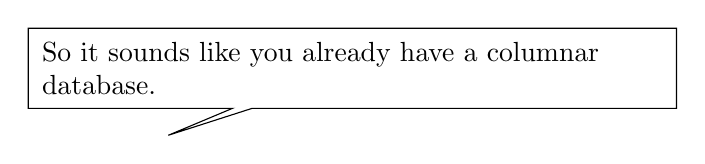
\begin{tikzpicture}[>=latex]
\node[rectangle callout, draw, inner sep=5 pt, callout relative pointer={(200:1 cm)}, text width=0.65\linewidth] {So it sounds like you already have a columnar database.};
\end{tikzpicture}

\vspace{0.25 cm}
\begin{uncoverenv}<2->
\hfill 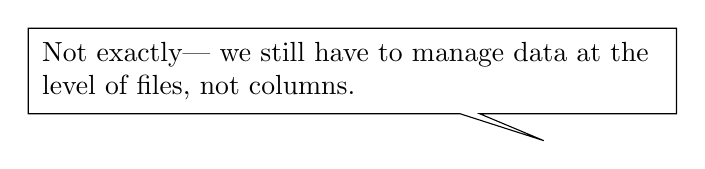
\begin{tikzpicture}[>=latex]
\node[rectangle callout, draw, inner sep=5 pt, callout relative pointer={(-200:-1 cm)}, text width=0.65\linewidth] {Not exactly--- we still have to manage data at the level of files, not columns.};
\end{tikzpicture}
\end{uncoverenv}

\vspace{0.25 cm}
\begin{uncoverenv}<3->
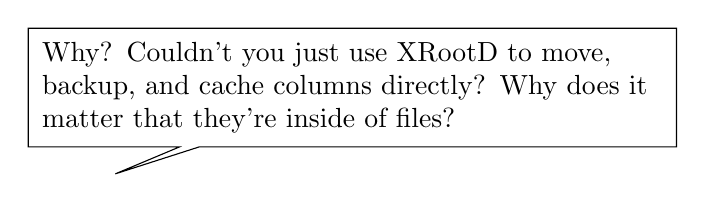
\begin{tikzpicture}[>=latex]
\node[rectangle callout, draw, inner sep=5 pt, callout relative pointer={(200:1 cm)}, text width=0.65\linewidth] {Why? Couldn't you just use XRootD to move, backup, and cache columns directly? Why does it matter that they're inside of files?};
\end{tikzpicture}
\end{uncoverenv}

\vspace{0.25 cm}
\begin{uncoverenv}<4->
\hfill 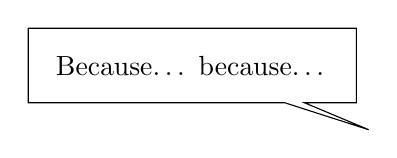
\begin{tikzpicture}[>=latex]
\node[rectangle callout, draw, inner sep=10 pt, callout relative pointer={(-200:-1 cm)}] {Because\ldots\ because\ldots};
\end{tikzpicture}
\end{uncoverenv}
\end{frame}

\begin{frame}{Proof that it matters: CMS NanoAOD}
\vspace{0.5 cm}
\textcolor{darkblue}{\underline{Stated goal:}} {to serve 30--50\% of CMS analyses with a single selection of columns.}

\vspace{0.5 cm}
Painful decisions need to be made to keep disk size down to 1--2~kB/event, to make data access faster for 50\% of analyses while excluding others.

\vspace{0.5 cm}
\begin{columns}
\column{0.55\linewidth}
\begin{center}
\uncover<2->{If we could really manage data at the columnar level, we could just put the most frequently used 1--2~kB/event in warm storage and the other 40~kB/event in cold storage.}
\end{center}

\column{0.4\linewidth}
\begin{center}
\uncover<3->{Instead, we'll probably put the whole small copy (NanoAOD) in warm storage and the whole large copy (MiniAOD) in cold storage.}
\end{center}
\end{columns}
\end{frame}

\begin{frame}{}
\vspace{0.5 cm}
\begin{center}
\large Except for the simplest cases, we can't pull out individual branches \\ and manage them on their own, because only ROOT knows how to interpret \\ a branch's relationship with other branches.

\vspace{1 cm}
\uncover<2->{BulkIO can extract branch data as arrays, bypassing the reconstruction into events, but only for certain branch types (``non-destructively serialized'').}
\end{center}
\end{frame}

\begin{frame}[fragile]{What would it look like if we could?}
\begin{minted}{sql}
CREATE TABLE derived_data AS
    SELECT pt, eta, phi, deltaphi**2 + deltaeta**2 AS deltaR
    FROM original_data WHERE deltaR < 0.2;
\end{minted}

creates a new {\tt derived\_data} table from {\tt original\_data}, but {\it links}, rather than {\it copying}, {\tt pt}, {\tt eta}, and {\tt phi}.\footnote{Implementation dependent, but common. ``{\tt WHERE}'' selection may be implemented with a stencil.}

\vspace{0.25 cm}
\uncover<2->{If {\tt original\_data} is deleted, the database would not delete {\tt pt}, {\tt eta}, and {\tt phi}, as they're in use by {\tt derived\_data}.}

\vspace{0.5 cm}
\uncover<3->{\textcolor{darkblue}{\underline{For data management,}} this is a flexible system, as columns are a more granular unit for caching and replication.}

\vspace{0.25 cm}
\uncover<4->{\textcolor{darkblue}{\underline{For users,}} there is little cost to creating derived datasets, multiple versions of corrections and cuts.}
\end{frame}

\begin{frame}{}
\vspace{1 cm}
\begin{center}
\Large \textcolor{darkblue}{\underline{Idea \#1}.} Cast data from ROOT files into a well-known \\ standard for columnar, hierarchical data; manage those \\ columns individually in an object store like Ceph.
\end{center}

\begin{enumerate}
\item<2-> \textcolor{darkblue}{Apache Arrow} is one such standard. It's similar to ROOT's splitting format but splits at all levels of depth.
\item<3-> \textcolor{darkblue}{PLUR or PLURP}. My subset of the above with looser rules about how data may be referenced. Stands for {\bf Primitives}, {\bf Lists}, {\bf Unions}, {\bf Records}, and maybe {\bf Pointers} (extension beyond Arrow).
\end{enumerate}

\vspace{0.25 cm}
\begin{center}
\uncover<4->{\Large ``Datacenter groks the data.''}
\end{center}
\end{frame}

\begin{frame}{}
\vspace{1 cm}
\begin{center}
\Large \textcolor{darkblue}{\underline{Idea \#2} (this talk).} 
\end{center}

\begin{enumerate}
\end{enumerate}

\vspace{0.25 cm}
\begin{center}
\uncover<4->{\Large ``ROOT eats the world.''}
\end{center}
\end{frame}



\end{document}
